\chapter{Results and Evaluation}

In this chapter, we assess the potential benefit of using SecureWilly in docker projects. Through a variety of experiments, we display the results of SecureWilly's execution we examine the profiles produced and we evaluate the performance and the scalability of our software.

\section{Experimental Evaluation}
\subsection{Benchmarks}
SecureWilly has been tested on creating AppArmor profiles for a set of multi-service projects provided by CloudSuite, a benchmark suite for cloud services. \cite{cloudsuite} The benchmarks are based on real-world software stacks and represent real-world setups. 

\begin{description}[style=nextline]
\item[Media Streaming]
One of the benchmarks of Cloudsuite that was used in the experimental evaluation was media-streaming. This benchmark uses the Nginx web server as a streaming server for hosted videos of various lengths and qualities. The client, based on httperf's wsesslog session generator, generates a request mix for different videos, to stress the server. \cite{mediastr}

The benchmark has two tiers: the server and the clients. The server runs Nginx, and the clients send requests to stream videos from the server. Each tier has its own image which is identified by its tag.

The streaming server requires a video dataset to serve and a synthetic dataset is generated, comprising several videos of different lengths and qualities. A separate docker image that handles the dataset generation is provided, which is then used to launch a dataset container that exposes a volume containing the video dataset.

To facilitate the communication between the client(s) and the server, a docker network is built, and the launched containers were attached to it.

\item[Data-Caching]
Another benchmark of CloudSuite that was used in our experimental evaluation was data-caching. This benchmark uses the Memcached data caching server, simulating the behavior of a Twitter caching server using a twitter dataset. The metric of interest is throughput expressed as the number of requests served per second. The workload assumes strict quality of service guarantees. \cite{datacaching}

This benchmark features two tiers: the server(s), running Memcached, and the client(s), which request data cached on the Memcached servers. Each tier has its own image which is identified by its tag.

To facilitate the communication between the client(s) and the server, a docker network is built, and the launched containers were attached to it.
\end{description}

\subsection{Nextcloud}

Despite the fact that CloudSuite's benchmarks are based on real-world software, we considered testing a real program, which is widely used and a lot of users rely on docker images in order to run it, and exercise it first-hand. Our choice was Nextcloud.

Nextcloud is a suite of client-server software for creating and using file hosting services. It is free and open-source, which means that anyone is allowed to install and operate it on their own private server devices. \cite{wikinext}

Although it is true that Nextcloud offers a variety of operations, we will be using it in its simplest form, where Nextcloud is used to run a personal cloud storage service, making files accessible via the internet and sharing them with other users.

The services of Nextcloud's project in the particular example are two:
\begin{enumerate}
\item \textbf{db}, which is actually the database used for data storage - in our case, we chose a MySQL/MariaDB database
\item \textbf{nextcloud}, which is the server of this docker project
\end{enumerate}

The docker-compose file which was used as input to SecureWilly's UI is the following (options security\_opt and container name were added by SecureWilly):

\begin{lstlisting}[style=Dockerfile, caption={Nextcloud's docker-compose.yml}]
version: '3'

volumes:
     nextcloud_:
     db_:

services:
     db:
        container_name: db
        security_opt:
          - "apparmor:db_profile"
        image: mariadb:10
        command: --transaction-isolation=READ-COMMITTED --binlog-format=ROW
        restart: always
        volumes:
                - db_:/var/lib/mysql
        environment:
                - MYSQL_ROOT_PASSWORD=secret
                - MYSQL_PASSWORD=secret
                - MYSQL_DATABASE=nextcloud_
                - MYSQL_USER=willy
     nextcloud:
        container_name: nextcloud
        security_opt:
          - "apparmor:nextcloud_profile"
        image: nextcloud
        ports:
                - 8080:80
        links:
                - db
        volumes:
                - nextcloud_:/var/www/html
                - /home/ubuntu/SecureWilly/Nextcloud/data:
					/var/www/html/data
        environment:
                - NEXTCLOUD_ADMIN_USER=willy
                - NEXTCLOUD_ADMIN_PASSWORD=secret
                - NEXTCLOUD_TABLE_PREFIX=nc_
                - NEXTCLOUD_DATA_DIR=/var/www/html/data
        restart: always
\end{lstlisting}

The Nextcloud installation and all data beyond what lives in the database (file uploads, etc) is stored in the docker volume /var/www/html. The docker daemon will store that data within the docker directory /var/lib/docker/volumes/. This keeps data persistent, meaning it is saved even if the container crashes, is stopped or deleted.

The volumes used in the yml file are the following:
\begin{itemize}
\item /var/www/html: Main folder, needed for updating
\item /var/www/html/data: The actual data of your Nextcloud
\item /var/lib/mysql: Database's volume
\end{itemize}

The test plan, which we provided as input, was minimal as it included some configuration commands for nextcloud's server and uploading a file to the cloud storage:

\begin{lstlisting}[style=bashscript, caption={Test plan used in Nextcloud's project}]
#Clear data directory if it exists and chown it to www-data, as configured in Nextcloud
sudo rm -r /home/ubuntu/SecureWilly/Nextcloud/data
mkdir /home/ubuntu/SecureWilly/Nextcloud/data
sudo chown www-data:www-data /home/ubuntu/SecureWilly/Nextcloud/data

#Start the containers
docker-compose up -d

#Wait some time for the database to be configured
sleep 60

#Check server's status
docker exec -u www-data nextcloud php occ status > answer
answer=$(cat answer | grep 'Nextcloud is not installed')
while [ -z "$answer" ]
do
        rm answer
        docker exec -u www-data nextcloud php occ status > answer
        answer=$(cat answer | grep 'Nextcloud is not installed')
done
rm answer

#Configure nextcloud, when the server is up
docker exec -u www-data nextcloud php occ maintenance:install --database "mysql" --database-name "nextcloud_" --database-host "db" --database-user "willy" --database-pass "secret" --admin-user "willy" --admin-pass "secret"

#Create a file in local data directory
sudo touch /home/ubuntu/SecureWilly/Nextcloud/data/willy/files/HelloFromTheOtherSide

#Use occ files:scan to make it visible to the web interface
docker exec -u www-data nextcloud php occ files:scan --all

#Stop the containers when you're finished
docker kill nextcloud
docker kill db
\end{lstlisting}

\subsection{Evaluation of the profiles produced}

In the following instances, the benchmarks were executed, having one client and one server. SecureWilly produced one profile for each of the services of every benchmark.
\hfill\break

\underline{Rules per run}
\hfill\break

In Figure 5.1, a line graph illustrates the amount of rules of each service's profile over the test plan runs, referring to media streaming benchmark.

\begin{figure}[h!]
  \centering
   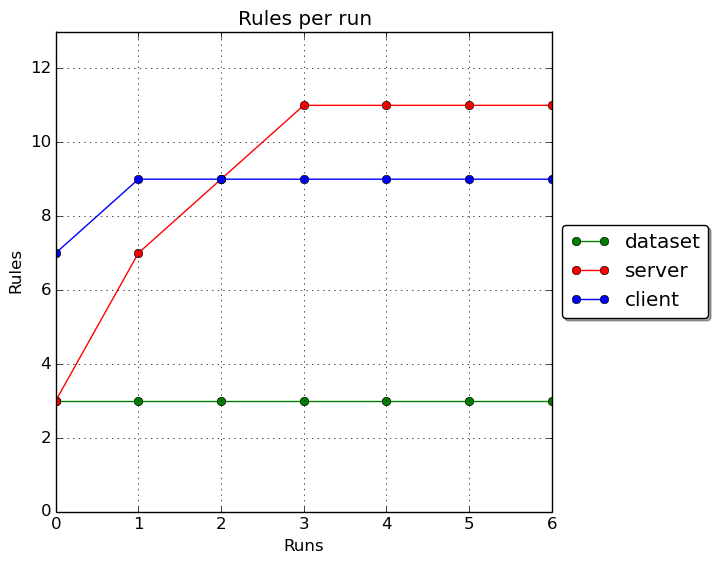
\includegraphics[width=0.8\linewidth]{./figures/mediastreaming/rules.png}
   \caption{Media Streaming: Rules per run for each service}
\end{figure}

All of the services start with non-zero amount of rules, which derives from static analysis's preliminary profiles.

We observe that most of the services had a gradual increase in their AppArmor profiles' rules, except for dataset, which starts with a preliminary profile of three rules and remains stable for the rest of the runs. This behaviour of dataset's profile is expected as the corresponding container does not execute any operations, but it only exists in order to expose a volume.

Server's and client's profiles follow a similar escalation, as they both rise to a point and then stabilize over the last runs. The rising derives from the first complain runs, in which rules are extracted gradually, as the addition of some rules leads to new system logs. While the first runs are crucial, as the most part of the rules are extracted over the first runs, the logs become gradually fewer over the last runs until all actions are allowed, and this explains the final stability of the profiles after some runs, shown in the graph.

It appears that there is a threshold in runs, which represents the minimum number of runs which have to be executed, until a profile stabilizes over runs.

Figure 5.2 shows the corresponding line graph to data-caching benchmark.

\begin{figure}[h!]
  \centering
   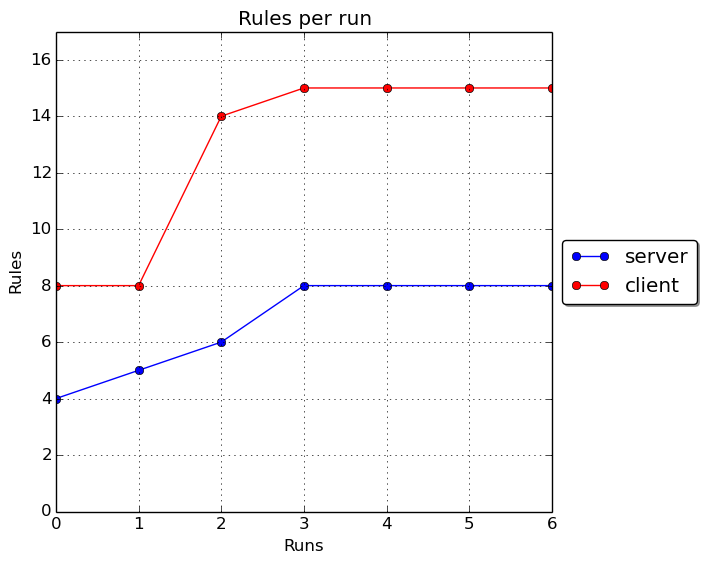
\includegraphics[width=0.8\linewidth]{./figures/datacaching/rules.png}
   \caption{Data Caching: Rules per run for each service}
\end{figure}


\hfill\break
\underline{Types of rules in final profile}
\hfill\break

The next step of the rules' analysis, was to identify which types of rules are encountered in our profiles. Figures 5.2, 5.3 and 5.4 shows a bar graph of the types of different rules used in the final AppArmor profile of each service. 

%\begin{textblock*}{18cm}(0.1cm,6.4cm) % {block width} (coords)
%\begin{figure}
%  \begin{minipage}[H!]{0.55\textwidth}
%    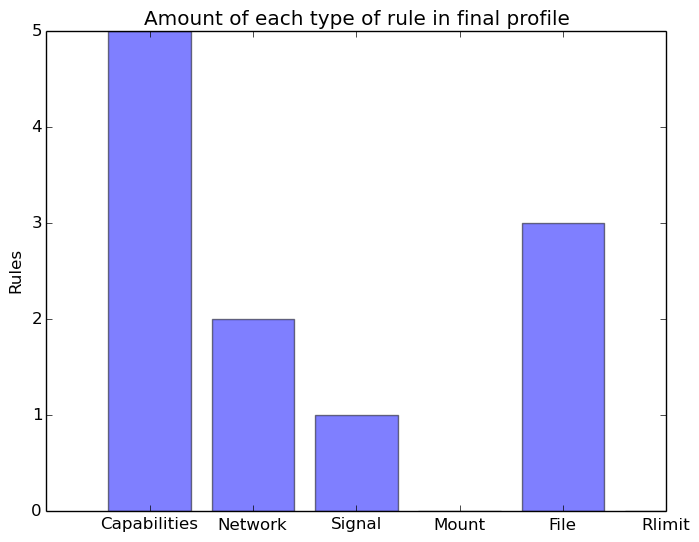
\includegraphics[width=\textwidth]{./figures/mediastreaming/Barfinal_cloudsuitemedia-streamingserver.png}
%    \caption{Server's types of rules}
%  \end{minipage}
%  \begin{minipage}[H!]{0.55\textwidth}
%    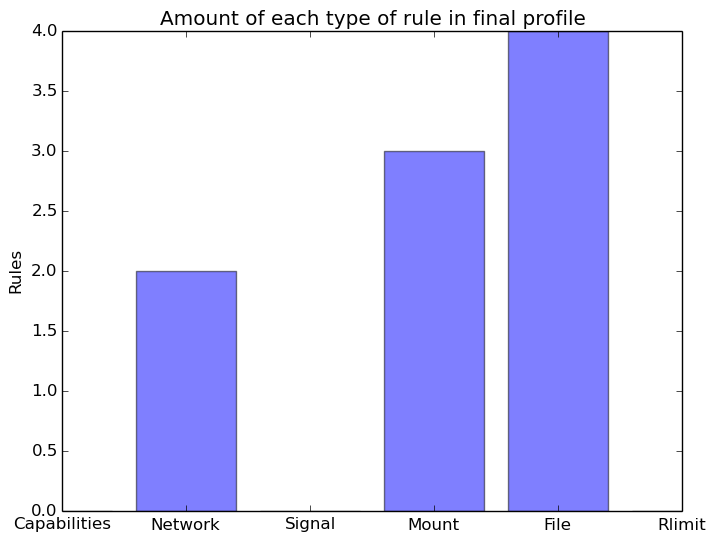
\includegraphics[width=\textwidth]{./figures/mediastreaming/Barfinal_cloudsuitemedia-streamingclient.png}
%    \caption{Client's types of rules}
%  \end{minipage}
%\end{figure}
%\end{textblock*}

\hfill\break\hfill\break\hfill\break\hfill\break\hfill\break\hfill\break\hfill\break\hfill\break\hfill\break\hfill\break\hfill\break\hfill\break\hfill\break\hfill\break\hfill\break\hfill\break\hfill\break

\begin{figure}[h!]
  \centering
   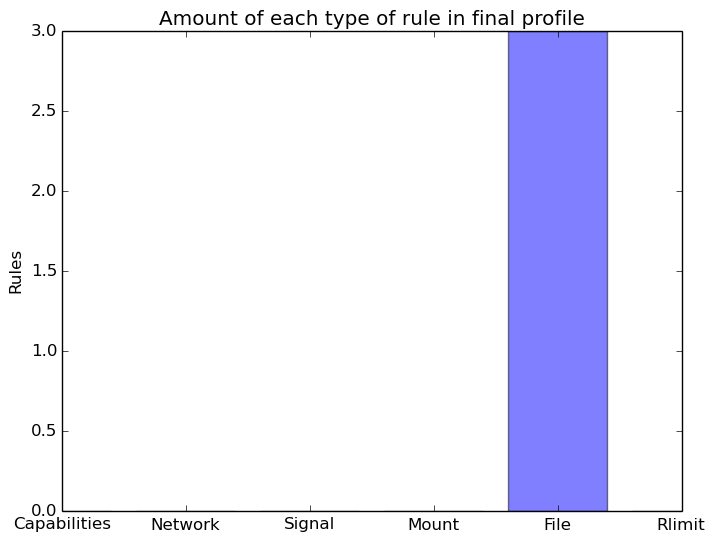
\includegraphics[width=0.64\linewidth]{./figures/mediastreaming/Barfinal_cloudsuitemedia-streamingdataset.png}
   \caption{Dataset's types of rules}
\end{figure}

The above bar graphs show that each profile describes perfectly the role of the service and the operations of its task.

In server's profile, the graph shows that a server has more capabilities rules than other types. This derives from the fact that a server commits several actions in order to serve the clients, and thus it is expected to need some capabilities. The file rules can derive from file access the server needs, but not from volumes since there are no mount rules extracted. Network rules are extracted for the internal communication of the services and lastly, one signal rule, which is needed in order to send a SEGKILL/SIGTERM to the server, since it is running as a daemon.

In client's profile, it appears that client had bind volumes, since there are mount rules and the corresponding file rules. File rules are more, because the preliminary profile's rules are added to them. Moreover, client also needs some network rules in order to communicate with the server.

As it is expeted, dataset only needs some file rules which are the ones of the preliminary profile, as its container will not commit any actions.

In the light of the above, it is clear that the AppArmor profile that are produced by SecureWilly are adjusted completely to the docker project and are closely tied with their tasks. That means they are efficient and secure, since they allow to the docker project to run unhinderedly, but all redundant actions will be denied.\\

\underline{Types of rules per run}
\hfill\break

Let's see how the rules of each type increment over the runs of the test plan.

\begin{figure}[h!]
  \centering
   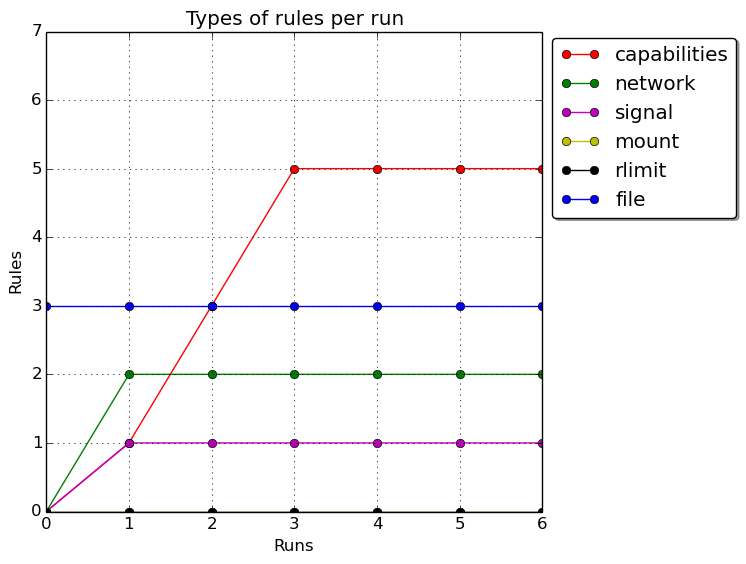
\includegraphics[width=0.64\linewidth]{./figures/mediastreaming/types_cloudsuitemedia-streamingserver.png}
   \caption{Server's types of rules per run}
\end{figure}

\begin{figure}[h!]
  \centering
   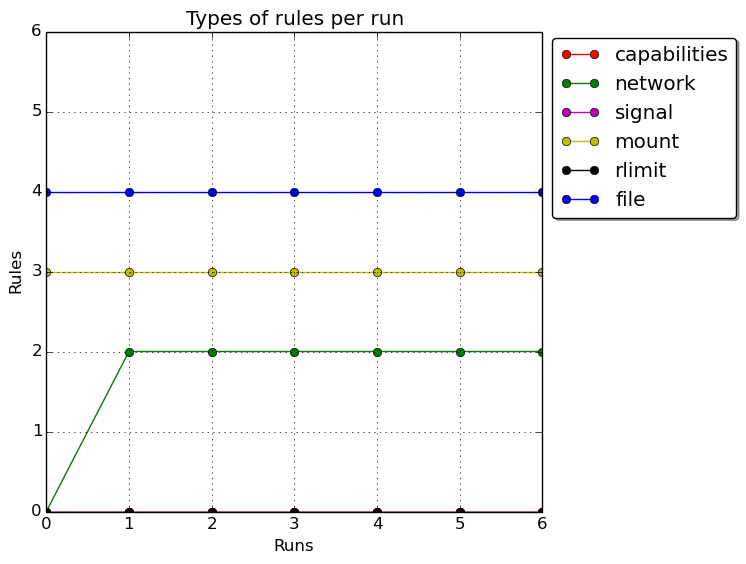
\includegraphics[width=0.64\linewidth]{./figures/mediastreaming/types_cloudsuitemedia-streamingclient.png}
   \caption{Client's types of rules per run}
\end{figure}

\begin{figure}[h!]
  \centering
   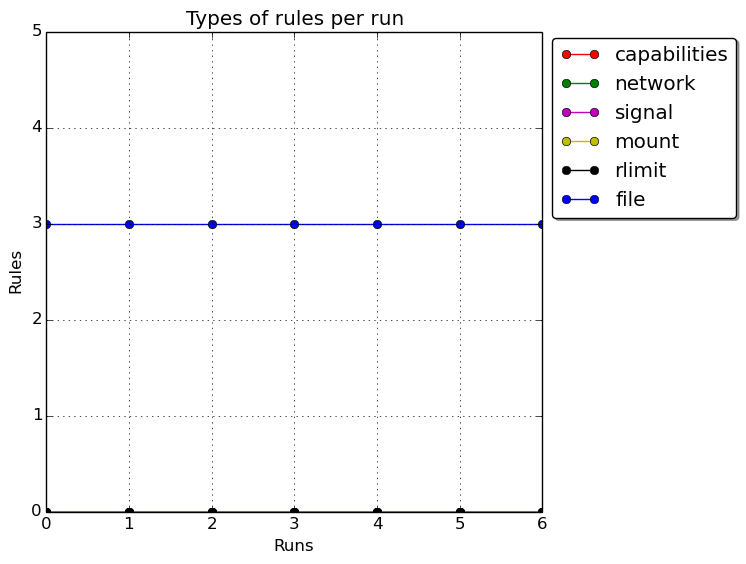
\includegraphics[width=0.64\linewidth]{./figures/mediastreaming/types_cloudsuitemedia-streamingdataset.png}
   \caption{Dataset's types of rules per run}
\end{figure}
